\section{Preliminaries: Probability Theory}
For this course, we will only be concerned with discrete probabilities. This section formalizes some notions you should already be familiar with: probability spaces, events and probability distributions.

\begin{definition}[Probability space]
A (discrete) probability space $(\Omega, \mathcal{F}, P)$ consists of a
discrete, non-empty \emph{sample space} $\Omega$, an \emph{event space}
$\mathcal{F} \subseteq \mathcal{P}(\Omega)$ and a \emph{probability measure} $P$ which is a function $P : \Omega \to \R_{\geq 0}$ that satisfies
\[
\sum_{\omega \in \Omega} P(\omega) = 1.
\]
\end{definition}
The event space $\mathcal{F}$ is required to be non-empty and closed under
intersection, union and complements. For convenience, we will most
often assume that $\mathcal{F}$ equals the powerset
$\mathcal{P}(\Omega)$ of $\Omega$, i.e.\ it
contains all
possible subsets of events, and therefore fulfils the required properties.

\begin{definition}[Event]\label{def:event}
An event $\evA$ is an element of the event space $\mathcal{F}
\subseteq \mathcal{P}(\Omega)$, i.e.\ a subset $\evA$ of the sample space $\Omega$. Its probability is defined as
\[
P[\evA] := \sum_{\omega \in \evA} P(\omega),
\]
where by convention $P[\emptyset] = 0$.
\end{definition}
As a notational convention, we write $P[\evA,\evB]$ for $P[\evA \cap \evB]$, and $P[\overline\evA]$ for $P[\Omega\backslash\evA]$.

\begin{exercise}
Prove the following identities (for arbitrary events $\evA, \evB \subseteq \Omega$):
\setlength{\abovedisplayskip}{0pt}
\setlength{\belowdisplayskip}{0pt}
\setlength{\abovedisplayshortskip}{0pt}
\setlength{\belowdisplayshortskip}{0pt}
\begin{align}
P[\overline{\evA}] &= 1 - P[\evA]\\
P[\evA \cup \evB] &= P[\evA] + P[\evB] - P[\evA, \evB]\\
P[\evA] &= P[\evA, \evB] + P[\evA, \overline\evB].
\end{align}
\end{exercise}
It is often useful to consider the probability of an event \emph{given} that some other event happened:
\begin{definition}[Conditional probability]\label{def:conditional-probability}
For events $\evA$ and $\evB$ with $P[\evA] > 0$, the conditional probability of $\evB$ given $\evA$ is defined as
\[
P[\evB | \evA] := \frac{P[\evA,\evB]}{P[\evA]} \, .
\]
\end{definition}
\begin{example}[Fair die]\label{ex:fair-die}
We throw a six-sided fair die once, and consider the number that comes
up. The sample space for this experiment is $\Omega =
\set{1,2,3,4,5,6}$, with event space $\mathcal{F} = \mathcal{P}(\Omega)$ and probability measure $P[i] =
\frac{1}{|\Omega|} = \frac{1}{6}$ for all $i \in \Omega$ (this is a
\term{uniform} probability measure). Consider the events $\evA = \set{2,4,6}$ and $\evB = \set{3,6}$.
Using the formulas in Definitions~\ref{def:event} and~\ref{def:conditional-probability}, we can compute the following probabilities:
\begin{align*}
P[\evA] &= \frac{1}{2} &\mbox{(the outcome is even)}\\
P[\evB] &= \frac{1}{3}&\mbox{(the outcome is a multiple of 3)}\\
P[\evA, \evB] &= P[\set{6}] = \frac{1}{6} & \mbox{(the roll is even \emph{and} a multiple of 3)}\\
P[\evA | \evB] &= \frac{1/6}{1/3} = \frac{1}{2} & \mbox{(the roll is even, \emph{given} that it is a multiple of 3)}\\
P[\evB | \evA] &= \frac{1/6}{1/2} = \frac{1}{3}& \mbox{(the roll is a multiple of 3, \emph{given} that it is even)}\\
\end{align*}
This example shows that in general, $P[\evA | \evB]$ is \emph{not
  equal} to $P[\evB | \evA]$.
\end{example}

\begin{definition}[Discrete Random Variable (RV)]
Let $(\Omega, \mathcal{F}, P)$ be a discrete probability space. A
random variable $X$ is a function $X : \Omega \to \mathcal{X}$ where
$\mathcal{X}$ is a set, and we may assume it to be discrete.
\end{definition}
A \emph{real} random variable is one whose image is contained in $\mathbb{R}$. A (The \emph{image} and the \emph{range} of a random variable $X$ are given by the image and the range of $X$ in the function-theoretic sense.) The image of a \emph{binary} random variable is a set $\set{x_0, x_1}$ with only two elements.

\begin{definition}[Probability distribution]
Let $X$ be a random variable. The probability distribution of $X$ is the function $P_X : \mathcal{X} \to [0,1]$ defined as
\[
P_X(x) := P[X = x],
\]
where $X = x$ denotes the event $\Set{\omega \in \Omega}{X(\omega) = x}$.
\end{definition}
Alternatively, one can write $P_X(x) = P(X^{-1}(x))$ to express that the
probability of $x$ is precisely the $P$-measure of the pre-image of $x$
under the random variable $X$.

\begin{exercise}
Verify that $(\mathcal{X},
\mathcal{P}(\mathcal{X}), P_X)$ is itself a probability space.
\end{exercise}

We say that $P_X$ is a \term{uniform} distribution if the associated
probability measure is uniform, i.e. $P_X(x) =
\frac{1}{|\mathcal{X}|}$. The \term{support} of a random variable or a
probability distribution is
defined as $\supp(P_X) := \{x \in \mathcal{X} \mid P_X(x) > 0\}$, the
points of the range which have strictly positive probability. We often
slightly abuse notation and write $\supp(X)$ instead.

When given two or more random variables defined on the same probability space, we can consider the probability that each of the variables take on a certain value:

\begin{definition}[Joint probability distribution]
Let $X$ and $Y$ be two random variables defined on the same probability space, with respective ranges $\mathcal{X}$ and $\mathcal{Y}$. The pair $XY$ is a random variable with probability distribution $P_{XY} : \mathcal{X} \times \mathcal{Y} \to [0,1]$ given by
\[
P_{XY}(x,y) := P[X = x, Y = y].
\]
\end{definition}
This definition naturally extends to three and more random variables. Unless otherwise stated, a collection of random variables is assumed to be defined on the same (implicit) probability space, so that their joint distribution is always well-defined.

If $P_{XY} = P_X \cdot P_Y$, in the sense that $P_{XY}(x,y) = P_X(x)P_Y(y)$ for all $x \in \mathcal{X}$ and $y 
\in \mathcal{Y}$, then the random variables $X$ and $Y$ are said to be \term{independent}. If a set of variables $X_1, ..., X_n$ are all mutually independent and all have the same distribution (i.e. $P_{X_i} = P_{X_j}$ for all $i,j$), then they are \term{independent and identically distributed}, or \term{i.i.d.}

From a joint distribution, we can always find out the ``original'' (or \term{marginal}) distribution of one of the random variables (for example, $X$) by \term{marginalizing} out the variable that we want to discard (for example, $Y$):
\begin{align}
P_X(x) = \sum_{y \in \mathcal{Y}} P_{XY}(x,y).
\end{align}
This marginalization process also works with more than two random variables.

Like events, probability distributions can also be conditioned on
probabilistic events:
\begin{definition}[Conditional probability distribution]
If $\evA$ is an event with $P[\evA] > 0$, then the conditional probability distribution of $X$ given $\evA$ is given by
\[
P_{X|\evA}(x) = \frac{P[X=x, \evA]}{P[\evA]}.
\]
If $Y$ is another random variable and $P_Y(y) > 0$, then we write
\[
P_{X | Y}(x| y) := P_{X | Y = y}(x) = \frac{P_{XY}(x,y)}{P_Y(y)}
\]
for the conditional distribution of $X$, given $Y = y$.
\end{definition}
Note that again, both $(\mathcal{X},P_{X | \evA})$ and $(\mathcal{X},P_{X| Y=y})$ themselves form probability spaces. Note also that if $X$ and $Y$ are independent, then
\begin{align}
P_{X | Y}(x |y) = \frac{P_{XY}(x,y)}{P_Y(y)} = \frac{P_X(x) \cdot P_Y(y)}{P_Y(y)} = P_X(x),
\end{align}
which aligns well with our intuition of independent variables: the distribution of $X$ remains unchanged when $Y$ is fixed to a specific value.

\begin{example}[Fair die (continued)]
Consider again the throw of a six-sided fair die as in Example~\ref{ex:fair-die}. Let the random variable $X$ describe the number of integer divisors for the outcome, that is
\[X(1) = 1 \ \ \ \ \ X(2) = 2 \ \ \ \ \ X(3) = 2 \ \ \ \ \ X(4) = 3 \ \ \ \ \ X(5) = 2 \ \ \ \ \ X(6) = 3
\]
$X$ is a real random variable, with range $\mathcal{X} = \set{1,2,3}$. The associated probability distribution is
\[P_X(1) = P[\set{1}] = \frac{1}{6}, \ \ \ \ \ \ \ \ \ \ P_X(2) = P[\set{2,3,5}] = \frac{1}{2}, \ \ \ \ \ \ \ \ \ \ P_X(3) = P[\set{4,6}] = \frac{1}{3}.
\]
If we now condition on the event $\evA = \set{2,4,6}$ (the outcome being even), we get that
\[P_{X | \evA}(1) = 0, \ \ \ \ \ \ \ \ \ \ P_{X | \evA}(2) = \frac{1}{3}, \ \ \ \ \ \ \ \ \ \ P_{X | \evA}(3) = \frac{2}{3}.
\]
\end{example}
If $X$ is a random variable and $f : \mathcal{X} \to \mathcal{Y}$ is a surjective function, then $f(X)$ is a random variable, defined by composing the map $f$ with the map $X$. Its image is $\mathcal{Y}$. Clearly,
\begin{align}
P_{f(X)}(y) = \sum_{x \in \mathcal{X} : f(x) = y} P_X(x).
\end{align}
For example, $1/P_X(X)$ denotes the real random variable obtained from another random variable $X$ by composing with the map $1/P_X$ that assigns $1/P_X(x) \in \mathbb{R}$ to $x \in \mathcal{X}$.

\begin{definition}[Expectation]
The expectation of a \emph{real} random variable $X$ is defined as
\[
\Exp[X] := \sum_{x \in \mathcal{X}} P_X(x) \cdot x.
\]
\end{definition}
Note that if $X$ is not real, then we can still consider the expectation of some function $f : \mathcal{X} \to \mathbb{R}$, where
\begin{align}
\Exp[f(X)] = \sum_{x \in \mathcal{X}} P_X(x) \cdot f(X).
\end{align}
\begin{definition}[Variance]
The variance of a \emph{real} random variable $X$ is defined as
\[
\Var[X] := \Exp[(X - \Exp[X])^2].
\]
\end{definition}
The variation is a measure for the deviation of the mean. Hoeffding's inequality (here stated for binary random variables) states that for a list of i.i.d. random variables, the average of the random variables is close to the expectation, except with very small probability. We state it here without proof.

\begin{theorem}[Hoeffding's inequality]
Let $X_1, ..., X_n$ be independent and identically distributed binary random variables with $P_{X_i}(0) = 1 - \mu$ and $P_{X_i}(1) = \mu$, and thus $\Exp[X_i] = \mu$. Then, for any $\delta > 0$
\[
P\left[\sum_i X_i > (\mu + \delta) \cdot n\right] \leq \exp(-2\delta^2n).
\]
\end{theorem}

\section{Some Important Distributions}
\begin{itemize}
\item
The distribution of a biased coin with probability $P_X(1)=p$ to land
heads, and a probability of $P_X(0)=1-p$ to land tails is called
\href{https://en.wikipedia.org/wiki/Bernoulli_distribution}{\term{Bernoulli($p$)} distribution}. Its entropy is given by the binary
entropy $h(p)$. The expected value is $\Exp[X]=p$ and the variance is
$\Var[X]=p(1-p)$.
\item
When $n$ coins $X_1, X_2, \ldots, X_n$ are flipped independently and
every $X_i$ is Bernoulli($p$) distributed, let $S=\sum_{i=1}^n X_i$ be
their sum, i.e.\ the number of heads in $n$ throws of a biased
coin. Then, $S$ has the \href{https://en.wikipedia.org/wiki/Binomial_distribution}{\term{binomial($n,p$)} distribution}:
\begin{align}
P_S(k) = \binom{n}{k} p^k (1-p)^{n-k} &\ \ \ \ \ \mbox{ where } k=0,1,2,\ldots,n
\, .\\
\intertext{
From simple properties of the expected value and variance, one can
show that $\Exp[S]=np$ and $\Var[S]=np(1-p)$.
\item
The
\href{https://en.wikipedia.org/wiki/Geometric_distribution}{\term{geometric($p$)}
  distribution} of a random variable $Y$ is defined as the number of
times one has to flip a Bernoulli($p$) coin before it lands heads:}
 P_Y(k) = (1-p)^{k-1} p &\ \ \ \ \ \mbox{ where } k=1,2,3,\ldots \, .\\
\intertext{
There is another variant of the geometric distribution used in the literature,
where one excludes the final success event of landing
heads in the counting:
}
P_Z(k) = (1-p)^k p \, &\ \ \ \ \ \mbox{ where } k=0,1,2,3,\ldots \, .
\end{align}
While the expected values are slightly different, namely
$\Exp[Y]=\frac{1}{p}$ and $\Exp[Z]=\frac{1-p}{p}$, their variances are
the same $\Var[Y]=\Var[Z]=\frac{1-p}{p^2}$.
\end{itemize}

\section{Jensen's Inequality}
In the following, let $\mathcal{D}$ be an interval in $\mathbb{R}$.

\begin{definition}[Convex and concave functions]
The function $f : \mathcal{D} \to \mathbb{R}$ is convex if for all $x_1, x_2 \in \mathcal{D}$ and all $\lambda \in [0,1] \subset \mathbb{R}$:
\[
\lambda f(x_1) + (1-\lambda)f(x_2) \geq f(\lambda x_1 + (1-\lambda)x_2).
\]
The function $f$ is \emph{strictly} convex if equality only holds when $\lambda \in \set{0,1}$ or when $x_1 = x_2$.
\\The function $f$ is (strictly) concave if the function $-f$ is (strictly) convex.
\end{definition}
Intuitively, a function is convex if any straight line drawn between two points $f(x_1)$ and $f(x_2)$ lies above the graph of $f$ entirely. For a concave function, such a line must lie entirely beneath the graph.
\begin{example}
The following functions are convex (for $c \in \mathbb{R}$):
\\
{
\centering
\begin{tabular}{ccccc}
\begin{tikzpicture}
	\begin{axis}[xmin=-2, xmax=2,ymin=0,ymax=2, ,axis x line=bottom, axis y line=center,ticks=none, x axis line style =-, y axis line style=-,width=4cm,height=3cm]
	\addplot[mark=none,domain=-2:2,color=ocre] {x^2};
	\end{axis}
\end{tikzpicture}%
	&
\begin{tikzpicture}
	\begin{axis}[xmin=-5, xmax=5,ymin=0,ymax=5, ,axis x line=bottom, axis y line=center,ticks=none, x axis line style =-, y axis line style=-,width=4cm,height=3cm]
	\addplot[mark=none,domain=-5:5,color=ocre] {exp(-x)};
	\end{axis}
\end{tikzpicture}%
	&
\begin{tikzpicture}
	\begin{axis}[xmin=0, xmax=3,ymin=-1.5,ymax=2, ,axis x line=center, axis y line=left,ticks=none, x axis line style =-, y axis line style=-,width=4cm,height=3cm]
	\addplot[mark=none,domain=0:5,color=ocre] {ln(1/x)/ln(2)};
	\end{axis}
\end{tikzpicture}%
	&
\begin{tikzpicture}
	\begin{axis}[xmin=0, xmax=3,ymin=-1.5,ymax=2, ,axis x line=center, axis y line=left,ticks=none, x axis line style =-, y axis line style=-,width=4cm,height=3cm]
	\addplot[mark=none,domain=0:5,color=ocre] {x*ln(x)/ln(2)};
	\end{axis}
\end{tikzpicture}%
	&
\begin{tikzpicture}
	\begin{axis}[xmin=0, xmax=3,ymin=0,ymax=2, ,axis x line=bottom, axis y line=center,ticks=none, x axis line style =-, y axis line style=-,width=4cm,height=3cm]
	\addplot[mark=none,domain=0:5,color=ocre] {1};
	\end{axis}
\end{tikzpicture}
	\\
	$x^2$ & $e^{-x}$ & $\log(1/x)$ & $x\cdot\log x$ & $c$\\
\end{tabular}
}
\\\\The following functions are concave (for $c \in \mathbb{R}$):\\
{
\centering
\begin{tabular}{ccc}
\begin{tikzpicture}
	\begin{axis}[xmin=0, xmax=3,ymin=-2,ymax=2, ,axis x line=center, axis y line=left,ticks=none, x axis line style =-, y axis line style=-,width=4cm,height=3cm]
	\addplot[mark=none,domain=0:5,color=ocre] {ln(x)/ln(2)};
	\end{axis}
\end{tikzpicture}%
	&
\begin{tikzpicture}
	\begin{axis}[xmin=0, xmax=3,ymin=0,ymax=2, ,axis x line=center, axis y line=left,ticks=none, x axis line style =-, y axis line style=-,width=4cm,height=3cm]
	\addplot[mark=none,domain=0:5,color=ocre] {sqrt(x)};
	\end{axis}
\end{tikzpicture}%
	&
\begin{tikzpicture}
	\begin{axis}[xmin=0, xmax=3,ymin=0,ymax=2, ,axis x line=bottom, axis y line=center,ticks=none, x axis line style =-, y axis line style=-,width=4cm,height=3cm]
	\addplot[mark=none,domain=0:5,color=ocre] {1};
	\end{axis}
\end{tikzpicture}
	\\
	$\log x$ & $\sqrt{x}$ & $c$\\
\end{tabular}
}
\end{example}
The following establishes a more formal method of proving the convexity of a function.
\begin{proposition}
Let $f : \mathcal{D} \to \mathbb{R}$. If $\mathcal{D}$ is open, and for all $x \in \mathcal{D}$, the second order derivative $f''(x)$ exists and is non-negative (positive), then $f$ is convex (strictly convex).
\end{proposition}
We omit the proof, which can be found in, for example, \href{http://homepages.cwi.nl/~schaffne/courses/inftheory/2016/notes/CramerFehr.pdf}{[CF]} (Lemma 1).


\begin{theorem}[Jensen's inequality] Let $f : \mathcal{D} \to \mathbb{R}$ be a convex function, and let $n \in \mathbb{N}$. Then for any $p_1, ..., p_n \in \mathbb{R}_{\geq 0}$ such that $\sum_{i=1}^n p_i = 1$ and for any $x_1, ..., x_n \in \mathcal{D}$ it holds that
\[
\sum_{i=1}^n p_if(x_i) \geq f\left(\sum_{i=1}^np_ix_i\right).
\]
If $f$ is strictly convex and $p_1, ..., p_n > 0$, then equality holds iff $x_1 = \cdots = x_n$.

In particular, if $X$ is a real random variable whose image $\mathcal{X}$ is contained in $\mathcal{D}$, then
\[
\Exp[f(X)] \geq f(\Exp[X]),
\]
and if $f$ is strictly convex, equality holds iff there is a $c \in \mathcal{X}$ such that $X = c$ with probability 1.
\end{theorem}
\begin{proof}
The proof is by induction. The case $n=1$ is trivial, and the case $n=2$ is identical to the very definition of convexity. Suppose that we have already proved the claim up to $n-1 \geq 2$. Assume, without loss of generality, that $p_n < 1$. Then:
\begin{align}
\sum_{i=1}^n p_i f(x_i) &= p_n f(x_n) + \sum_{i=1}^{n-1} p_i f(x_i)\nonumber\\
&= p_n f(x_n) + (1-p_n)\sum_{i=1}^{n-1} \frac{p_i}{1-p_n} f(x_i)\nonumber\\
&\geq p_n f(x_n) + (1-p_n)f\left(\sum_{i=1}^{n-1} \frac{p_i}{1-p_n} x_i\right) & \mbox{(induction hypothesis)}\nonumber\\
&\geq f\left(p_n x_n + (1-p_n)\sum_{i=1}^{n-1} \frac{p_i}{1-p_n} x_i\right) & \mbox{(definition of convexity)}\nonumber\\
&= f\left(p_n x_n + \sum_{i=1}^{n-1} p_i x_i\right)\nonumber\\
&= f\left(\sum_{i=1}^np_ix_i\right).
\end{align}
That proves the claim. As for the strictness claim, if $x_1, ..., x_n$ are not all identical, then either $x_1, ..., x_{n-1}$ are not all identical and the first inequality is strict by induction hypothesis, or $x_1 = \cdots = x_{n-1} \neq x_n$ so that the second inequality is strict by the definition of convexity.
\end{proof}

\section{Shannon Entropy}
In this section, we explore a measure for the amount of uncertainty of random variables. Consider some probabilistic event $\evA$ that occurs with probability $P[\evA]$ for some probability measure $P$. The \term{surprisal value} $\log \frac{1}{P[\evA]}$ indicates how surprised we should be when the event $\evA$ occurs: events with small probabilities yield high surprisal values, and vice versa. An event that occurs with certainty ($P_X(\evA) = 1$) yields a surprisal value of 0. For a random variable $X$, we consider the {\em expected} surprisal value to be an indicator of how much uncertainty is contained in the variable, or how much information is gained by revealing the outcome. This expected surprisal value is more commonly known as the (Shannon) entropy\footnote{Shannon once said: \it My greatest concern was what to call it. I thought of calling it {\em information}, but the word was overly used, so I decided to call it {\em uncertainty}. When I discussed it with John von Neumann, he had a better idea. Von Neumann told me: ``You should call it {\em entropy}, for two reasons. In the first place, your uncertainty function has been used in statistical mechanics under that name, so it already has a name. In the second place, and more important, nobody knows what entropy really is, so in a debate you will always have the advantage.''  } of a random variable:

\begin{definition}[Entropy]\label{def:entropy}
Let $X$ be a random variable with image ${\cal X}$. The
(Shannon) entropy $H(X)$ of $X$ is defined as
\[
H(X) := \Exp\Bigl[\log\frac{1}{P_X(X)}\Bigr] = \sum_{x\in {\cal X}} P_X(x) \cdot \log \frac{1}{P_X(x)} = -\sum_{x\in {\cal X}} P_X(x) \cdot \log P_X(x) \, ,
\]
with the convention that the $\log$ function represents the {\em binary} logarithm $\log_2$. As another convention, for $x \in  \cal X$ with $P_X(x) = 0$, the corresponding argument in the summation is declared~$0$ (which is justified by
taking a limit).%
\end{definition}
%
It is important to realize that the entropy of $X$ is a function (solely) of the {\em distribution} $P_X$ of $X$. However, it is customary to write $H(X)$ instead of the formally correct $H(P_X)$. 

%The entropy of $X$ can also be expressed as the expectation of the random variable $\log\bigl(1/P_X(X)\bigr)$: 
%$$
%H(X)= \Exp\Bigl[\log\frac{1}{P_X(X)}\Bigr] \, .
%$$

\begin{proposition}[Positivity]\label{prop:positivity}
Let $X$ be a random variable with image ${\cal X}$. Then
\[
0\leq H(X) \leq \log(|{\cal X}|).
\]
Equality on the left-hand side holds iff there exists $x\in {\cal
X}$ with $P_X(x)=1$ (and thus $P_X(x')=0$ for all $x' \neq x$). Equality on the right-hand side holds iff
$P_X(x)=1/|{\cal X}|$ for all $x\in {\cal X}$.
\end{proposition}

\begin{proof}
The function $f:
\R_{>0} \to \R$ defined by $y\mapsto \log y$ is strictly
 concave on $\R_{>0}$. Thus, by Jensen's inequality: 
\begin{align}
H(X)=\sum_{x\in {\cal X}} P_X(x) \cdot \log \frac{1}{P_X(x)}\leq
\log\bigl(\textstyle\sum_{x\in {\cal X}} 1\bigr)=\log(|{\cal X}|).
\end{align}
Furthermore, since we may restrict the sum to all $x$ with $P_X(x)>0$, equality holds if and only if  $\log(1/P_X(x)) = \log(1/P_X(x'))$, and thus $P_X(x) = P_X(x')$, for all $x,x' \in \cal X$. 

Finally, for the characterization of the lower bound, it is obvious that $H(X) = 0$ if $P_X(x) = 1$ for some $x$, and, on the other hand, if $H(X) = 0$ then for any $x$ with $P_X(x) > 0$ it must be that $\log(1/P_X(x)) = 0$ and hence $P_X(x) = 1$. 
\end{proof}

For a binary random variable $X$ with image ${\cal X} = \{x_0,x_1\}$ and probabilities $P_X(x_0) = p$ and $P_X(x_1) = 1-p$, we can write $H(X) = h(p)$, where $h$ denotes the binary entropy function:

\begin{definition}[Binary entropy function $h$]
The binary entropy function is defined for $0 < q < 1$ as 
\[
h(q) := q \log\frac{1}{q} + (1-q)\log\frac{1}{1-q},
\]
and is defined as $h(q) = 0$ for $q=0$ or $q=1$. The graph of $h$ on the interval $[0,1]$ is shown in Figure~\ref{fig:bin-entropy}.
\end{definition}
This binary entropy function is used, for example, to measure the entropy of a biased coin flip. 
\begin{figure}[h]
\centering\begin{tikzpicture}
\begin{axis}[xlabel={$p$},ylabel={$h(p)$},domain=0:1,samples=100, no markers,xtick={0,0.5,1}]
\addplot[ocre]{-1*x*ln(x)/ln(2) - (1-x)*ln(1-x)/ln(2)};
\end{axis}
\end{tikzpicture}
\caption{The binary entropy function $h$ as a function of the probability $p$.}\label{fig:bin-entropy}
\end{figure}

\begin{example}
Consider a random variable $X$ with $\mathcal{X} = \set{a,b,c}$ and $P_X(a) = \frac{1}{2}$, $P_X(b) = P_X(c) = \frac{1}{4}$. The entropy of $X$ is
\begin{align}
H(X) = \frac{1}{2} \log 2 + \frac{1}{4} \log 4 + \frac{1}{4} \log 4 = \frac{1}{2} + \frac{1}{2} + \frac{1}{2} = \frac{3}{2}.
\end{align}
Another approach to computing the entropy of $X$ by coming up with an appropriate underlying probability space $(\Omega,P)$: we toss a fair coin twice, giving $\Omega = \set{\mathsf{hh}, \mathsf{ht}, \mathsf{th}, \mathsf{tt}}$ and $P(\omega) = \frac{1}{4}$ for all $\omega \in \Omega$. The we define the function $X : \Omega \to \mathcal{X}$ as
\[
X(\mathsf{hh}) = X(\mathsf{ht}) = a, \ \ \ \ \ \ \ \ \ \ X(\mathsf{th}) = b, \ \ \ \ \ \ \ \ \ \ X(\mathsf{tt}) = c.
\]
This yields the correct distribution $P_X$. The following computation now leads to the entropy of $X$:
\begin{align}
H(X) = h\left(\frac{1}{2}\right) + \frac{1}{2}h(0) + \frac{1}{2}h\left(\frac{1}{2}\right) = \frac{3}{2}.
\end{align}
The first coin toss determines whether the outcome is $a$ (on heads $\mathsf{h}$) or something else (on tails $\mathsf{t}$). On heads, the second coin toss does not give any more information, whereas on tails, the second coin toss still decides between outcome $b$ and outcome $c$. In general, the entropy of a random variable with probabilities $p_1, ..., p_n$ can be expressed as
\begin{align}
H(p_1, ..., p_k, p_{k+1}, ..., p_n) &= h(p_1 + \cdots + p_k) +\nonumber\\
&\ \ \ \ \ (p_1 + \cdots + p_k) H\left(\frac{p_1}{p_1+\cdots+p_k} + \cdots + \frac{p_k}{p_1+\cdots+p_k}\right) +\nonumber\\
&\ \ \ \ \ (p_{k+1} + \cdots + p_n)H\left(\frac{p_{k+1}}{p_{k+1}+\cdots+p_n} + \cdots + \frac{p_n}{p_{k+1}+\cdots+p_n}\right).
\end{align}
\end{example}

\section{Conditional Entropy}
Let $X$ be a random variable and $\cal A$ an event. Applying Definition~\ref{def:entropy} to the conditional probability distribution $P_{X|\cal A}$ allows us to naturally define the entropy of $X$ conditioned on the event $\cal A$, which leads to the following notion:


\begin{definition}[Conditional entropy]\label{def:CondEntropy}
Let $X$ and $Y$ be random variables, with respective images ${\cal
X}$ and ${\cal Y}$. 
The conditional entropy $H(X|Y)$ of $X$
given $Y$ is defined as
\[
H(X|Y) := \sum_{y\in {\cal Y}} P_Y(y)\cdot H(X|Y\!=\!y) \, ,
\]
with the convention that the corresponding argument in the summation is~$0$ for $y \in  \cal Y$ with $P_Y(y)=0$, and where
\[
H(X|{\cal A}) := \sum_{x\in {\cal X}} P_{X|{\cal A}}(x)\cdot \log
\frac{1}{P_{X|{\cal A}}(x)}.
\]
\end{definition}
%
Note that conditional entropy $H(X|Y)$ is not the entropy of a probability
distribution but an expectation: the average uncertainty about $X$
when given $Y$. The following bound expresses that (on average!)\ additional information, i.e. knowing $Y$, can only {\em decrease} the uncertainty.

\begin{proposition}\label{prop:conditional-bounds}
Let $X$ and $Y$ be random variables with respective images ${\cal X}$ and $\cal Y$. Then
\[
0 \leq H(X|Y) \leq H(X)
\]
Equality on the left-hand side holds iff $X$ is determined by $Y$,
i.e., for all $y\in {\cal Y}$, there is an $x\in {\cal X}$ such that
$P_{X|Y}(x|y)=1$.
Equality on the right-hand side holds iff
$X$ and $Y$ are independent.
\end{proposition}
%
\begin{proof}
The lower bound follows trivially from the definition and from Proposition~\ref{prop:positivity}, and so does the characterization of when $H(X|Y) = 0$. For the upper bound, note that
\begin{align}
H(X|Y) = \sum_{y} P_Y(y) \sum_x P_{X|Y}(x|y) \log\frac{1}{P_{X|Y}(x|y)} = \sum_{x,y} P_{XY}(x,y) \log\frac{P_Y(y)}{P_{XY}(x,y)}
\end{align}
and
\begin{align}
H(X) = \sum_x P_{X}(x) \log\frac{1}{P_{X}(x)} = \sum_{x,y} P_{XY}(x,y) \log\frac{1}{P_{X}(x)}
\end{align}
where the last equality is derived by marginalization. Note that in both expressions, we may restrict the sum to those pairs $(x,y)$ with $P_{XY}(x,y) > 0$. 
Using Jensen's inequality, it follows that
\begin{align}
H(X|Y) - H(X) &= \sum_{x,y} P_{XY}(x,y)\log
\frac{P_X(x)P_Y(y)}{P_{XY}(x,y)} \nonumber \\
&\leq \log\Bigl( \sum_{x,y} P_X(x)P_Y(y) \Bigr) \leq \log\Bigl(\big(\sum_{x}P_X(x)\big)\big(\sum_{y}P_Y(y)\big)\Bigr) = \log 1 = 0 \, .
\end{align}
Note that in the second inequality, we replaced the summation over all $(x,y)$ with $P_{XY}(x,y) > 0$ by the summation over all $(x,y) \in {\cal X} \times {\cal Y}$. Inequality then follows by the monotonicity of the logarithm function.

For the first inequality, equality holds if and only if $P_{XY}(x,y) = P_X(x) P_Y(y)$ for all $(x,y)$ with $P_{XY}(x,y) > 0$, and for the second inequality, equality holds if and only if $P_{XY}(x,y) = 0$ implies $P_X(x) P_Y(y) = 0$ for any $x \in \cal X$ and $y \in \cal Y$. It follows that $H(X|Y) = H(X)$ if and only if $P_{XY}(x,y) = P_X(x) P_Y(y)$ for all $(x,y) \in {\cal X} \times {\cal Y}$. 
\end{proof}


\begin{proposition}[Chain Rule] 
Let $X$ and $Y$ be random variables. Then
\[
H(XY)= H(X) + H(Y|X) \, .
\]
\end{proposition}

\begin{proof}
The chain rule is a simple matter of rewriting:

\begin{align}
H(XY) &= -\sum_{x,y} P_{XY}(x,y)\log P_{XY}(x,y) \nonumber \\
&= -\sum_{x,y} P_{XY}(x,y)\log\bigl(P_X(x)P_{Y|X}(y|x)\bigr) \nonumber \\
&= -\sum_{x,y} P_{XY}(x,y) \log P_X(x)  -\sum_{x,y}
P_{XY}(x,y) \log P_{Y|X}(y|x) \nonumber \\
%&= -\sum_{x}P_X(x)\log P_X(x) -\sum_{x,y} P_{XY}(x,y) \log P_{Y|X}(y|x) \nonumber \\
&=  -\sum_{x}P_X(x)\log P_X(x) - \sum_{x} P_X(x)\sum_{y} P_{Y|X}(y|x) \log
P_{Y|X}(y|x) \nonumber \\
&= H(X) + H(Y|X) \, .
\end{align}
This was to be shown. 
\end{proof}
The following inequality, also known as the `independence bound', follows from the fact that $H(Y|X)\leq H(Y)$:
\begin{corollary}[Subadditivity]
\[
H(XY)\leq H(X)+H(Y) \, .
\]
Equality holds iff $X$ and $Y$ are independent.
\end{corollary}

Note that applying Definition~\ref{def:CondEntropy} to the conditional distribution $P_{XY|\cal A}$ naturally defines $H(X|Y,{\cal A})$, the entropy of $X$ given $Y$ and conditioned on the event $\cal A$. 
Since the entropy is a function of the distribution of a random variable, the chain rule also holds when conditioning on an event ${\cal A}$. Furthermore, it holds that
\begin{align}
H(X|YZ) = \sum_z P_Z(z) H(X|Y,Z\!=\!z) \, ,
\end{align}
which is straightforward to verify. With this observation, it is easy to see that the chain rule generalizes as follows. 

\begin{corollary}
Let $X$, $Y$ and $Z$ be random variables. Then
\[
H(XY|Z) = H(X|Z) + H(Y|XZ) \, .
\]
\end{corollary}%
Inductively applying the (generalized) chain rule implies that for any sequence $X_1,\ldots,X_n$ of random variables: 
\begin{align}
H(X_1\cdots X_n)= H(X_1) + H(X_2|X_1) + \cdots + H(X_n|X_{n-1}\cdots
X_1) \, .
\end{align}
%In particular,
%$$
%\sum_{i=1}^n H(X_1\cdots X_n)\leq \sum_{i=1}^n H(X_i).
%$$

\begin{example}\label{example:chain-rule}
Consider the binary random variables $X$ and $Y$, with joint distribution
\[
P_{XY}(00) = \frac{1}{2}, \ \ \ \ \ P_{XY}(01) = \frac{1}{4}, \ \ \ \ \ P_{XY}(10) = 0, \ \ \ \ \ P_{XY}(11) = \frac{1}{4}.
\]
By marginalization, we find that $P_X(0) = \frac{3}{4}$ and $P_X(1) = \frac{1}{4}$, while $P_Y(0) = P_Y(1) = \frac{1}{2}$. This allows us to make the following computations:
\begin{align}
H(XY) &= \frac{1}{2}\log 2 + \frac{1}{4} \log 4  + \frac{1}{4} \log 4 = \frac{3}{2}\\
H(X) &= h\left(\frac{1}{4}\right) = h\left(\frac{3}{4}\right) \approx 0.81\\
H(Y) &= h\left(\frac{1}{2}\right) = 1\\
H(X|Y) &= H(XY) - H(Y) = \frac{1}{2}\\
H(Y|X) &= H(XY) - H(X) \approx 0.69
\end{align}
We also could have computed $H(X|Y)$ and $H(Y|X)$ directly through the definition of conditional entropy.

Note that for this specific distribution, $H(X|Y=1) > H(X)$. It is important to remember that Proposition~\ref{prop:conditional-bounds} only holds on average, not for specific values of $Y$. Note also that in this example, $H(X|Y) \neq H(Y|X)$. 
\end{example}

\section{Mutual Information}
\begin{definition}[Mutual information]\label{def:mutual-information}
Let $X$ and $Y$ be random variables. The mutual information
$I(X;Y)$ of $X$ and $Y$ is defined as
\[
I(X;Y)= H(X) - H(X|Y).
\]
\end{definition}
%
Thus, in a sense, mutual information reflects the reduction in
uncertainty about $X$ when given $Y$. Note the following properties of the mutual information:
\begin{align}
I(X;Y) &= H(X) + H(Y) - H(XY) &\mbox{(by chain rule)}\\
I(X;Y) &= I(Y;X) &\mbox{(``symmetry")}\\
I(X;Y) &\geq 0 &\mbox{(by subadditivity)}\\
I(X;Y) &= 0 \mbox{ iff $X$ and $Y$ are independent}\\
I(X;X) &= H(X) &\mbox{(``self-information'')}
\end{align}

Applying Definition~\ref{def:mutual-information} to the conditional distribution $P_{XY|\cal A}$ naturally defines $I(X;Y|{\cal A})$, the mutual information of $X$ and $Y$ conditioned on the event $\cal A$.

\begin{definition}[Conditional mutual information]
Let $X,Y,Z$ be random variables. Then the conditional mutual
information of $X$ and $Y$ given $Z$ is defined as
\[
I(X;Y| Z) = \sum_z P_Z(z) I(X;Y|Z\!=\!z) \, ,
\]
with the convention that the corresponding argument in the summation is~$0$ for $z$ with $P_Z(z)=0$. 
\end{definition}
%
Conditional mutual information has properties similar to the ones we saw above:

\begin{align}
I(X;Y|Z) &= I(Y;X|Z)\\
I(X;Y|Z) &\geq 0\\
I(X;Y|Z) &= 0 \mbox{ iff $X$ and $Y$ are independent given $Z$}
\end{align}
Furthermore, the previous bounds $H(X) \geq 0$, $H(X|Y) \geq 0$, and  $I(X;Y) \geq 0$, can all be seen as special cases of $I(X;Y| Z) \geq 0$. These bounds, and any bound they imply, are called \term{Shannon inequalities}.

It is important to realize that $I(X;Y| Z)$ may be larger or smaller than (or equal to) $I(X;Y)$. 
The following is easy to verify (and is sometimes used as definition of $I(X;Y| Z)$). 
\begin{proposition}
Let $X,Y,Z$ be random variables. Then 
\[
I(X;Y| Z)= H(X|Z)- H(X|YZ) \, .
\]
\end{proposition}
%
By this result, we obtain: 


\begin{corollary}[Chain rule for mutual information]
Let $W,X,Y$ and $Z$ be random variables. Then
\[
I(WX;Y|Z) = I(X;Y|Z)+ I(W;Y|ZX) \, .
\]
\end{corollary}
\begin{proof}
The proof is a matter of writing out definitions and applying the generalized chain rule.
\begin{align}
I(WX;Y|Z) &= H(WX|Z) - H(WX|YZ)\nonumber\\
&= (H(X|Z) + H(W | XZ)) - (H(X|YZ) + H(W|XYZ))\nonumber\\
&= H(X|Z) - H(X|YZ) + H(W|XZ) - H(W|XYZ)\nonumber\\
&= I(X;Y|Z) + I(W;Y|XZ).
\end{align}
\end{proof}

\section{Relative entropy}
A measure that is related to the mutual information is the relative entropy: it reflects how different two distributions are:
\begin{definition}[Relative entropy]
The relative entropy (or: \term{Kullback leibner distance}) of two probability distributions $P$ and $Q$ over the same $\mathcal{X}$ is defined by
\[
D(P||Q) := \sum_{\substack{x \in \mathcal{X} \\ P(x) > 0}} P(x) \log \frac{P(x)}{Q(x)},
\]
where by convention, $\log\frac{p}{0} = \infty$ for all $p$.
\end{definition}
Note that if $Q(x) = 0$ for some $x$ with $P(x) > 0$, then $D(P||Q) = \infty$.

\begin{exercise}
Show that $I(X;Y) = D(P_{XY} || P_X \cdot P_Y)$. 
\end{exercise}
This exercise, combined with the equality condition in Theorem~\ref{thm:inf-ineq} below, shows that the mutual information is a measure of `how independent' the variables $X$ and $Y$ are: if $P_{XY} = P_X \cdot P_Y$, the variables are independent and their mutual information is zero.

\begin{theorem}[Information inequality]\label{thm:inf-ineq}
For any two probability distributions $P$ and $Q$ defined on the same $\mathcal{X}$,
\[
D(P||Q) \geq 0.
\]
Equality holds if and only if $P = Q$.
\end{theorem}
\begin{proof}
Left as an exercise. Hint: use Jensen's inequality.
\end{proof}



\section{Entropy Diagrams}\label{sec:Venn}
We finish this chapter by visually summing up the relations between entropy, joint entropy, conditional entropy, mutual information, and conditional mutual information. For two and three random variables, the relations between these different information-theoretic measures can be nicely represented by means of a Venn-diagram-like \term{entropy diagram}. The case of two random variables is illustrated in Figure~\ref{fig:entropy-diagram} (left). From the diagram, one can for instance easily read off the relations $H(X|Y) \leq H(X)$, $I(X;Y) = H(X) + H(Y) - H(XY)$ etc. The case of three random variables is illustrated in Figure~\ref{fig:entropy-diagram} (right). Also here, one can easily read off all the relations between the information-theoretic measures, like for instance $H(X|YZ) = H(X) -I(X;Z) - I(X;Y|Z)$, which is a relation that is otherwise maybe not immediately obvious.

\begin{figure}[H]
%\begin{center}
\ifpdf
\begin{minipage}[b]{6cm}
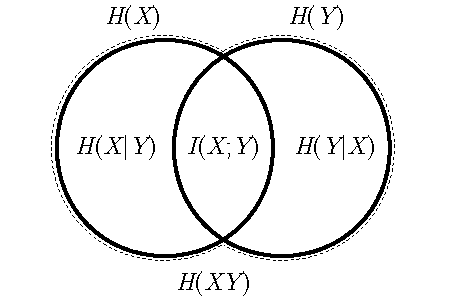
\includegraphics[width=6.5cm]{Venn1.pdf} \\[4ex]
\end{minipage}
\begin{minipage}[b]{6cm}
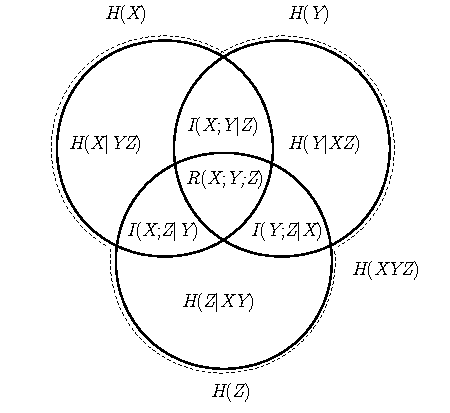
\includegraphics[width=8.5cm]{Venn2.pdf}
\end{minipage}
\else
\begin{minipage}[b]{6cm}
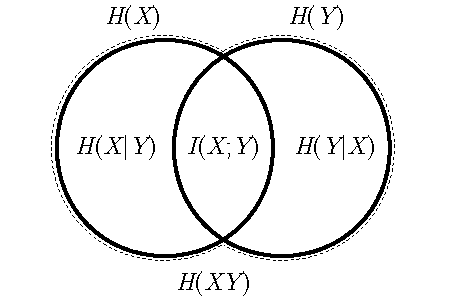
\includegraphics[width=6.5cm]{Venn1.eps} \\[4ex]
\end{minipage}
\begin{minipage}[b]{6cm}
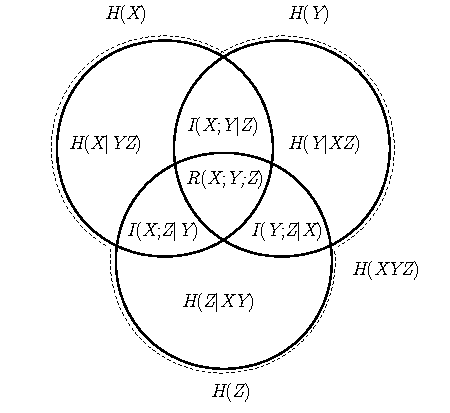
\includegraphics[width=8.5cm]{Venn2.eps}
\end{minipage}
\fi
%\end{center}
\vspace{-2ex}
\caption{Entropy diagram for two (left) and three (right) random variables. The areas encompassed by the dotted lines represent $H(XY)$ and $H(XYZ)$, respectively.}\label{fig:entropy-diagram}
\end{figure}

One subtlety with the entropy diagram for three random variables is that the ``area in the middle'', $R(X;Y;Z) = I(X;Y) - I(X;Y|Z)$, may be {\em negative}.



\section{Further Reading}
\begin{itemize}
\item Sections 2.1, 2.2, 3.1-3.3 of \CF
\item Sections 2.1, 2.2, 2.6 of \CT
\item For more background on probability theory, check for instance the \href{https://github.com/BasicProbability/LectureNotes/raw/master/fullscript/BasicProbabilityAndStatistics.pdf}{lecture
  script} of the Master of Logic course ``Basic Probability:Theory''
by Philip Schulz and Christian Schaffner.
\end{itemize}



%%% Local Variables:
%%% mode: latex
%%% TeX-master: "InfTheory3.tex"
%%% End: